\begin{figure}[t]
    \centering
    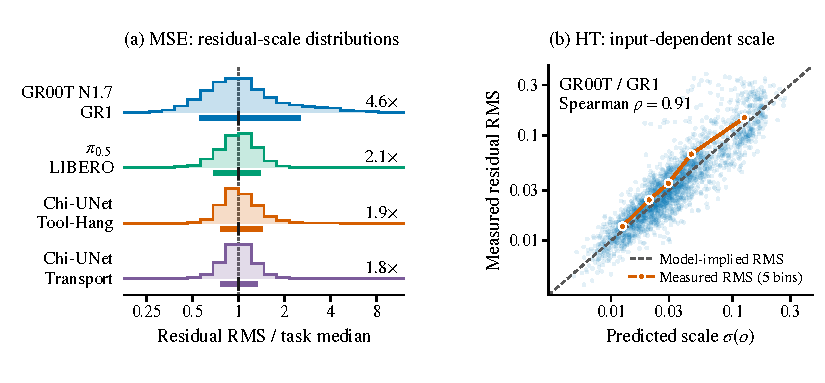
\includegraphics[width=\linewidth]{multiscale_rms.pdf}
    \caption{\textbf{Residual scales vary across demonstration inputs.}
    (a) MSE action-chunk residual RMS distributions, normalized by the median
    within each task and aggregated with equal task weights. Histograms use
    log-spaced bins and equal peak heights; bars mark the 10th--90th
    percentiles, with their ratios annotated.
    (b) In a separate GR1 HT probe, predicted scale tracks measured residual
    RMS ($\rho=0.91$). Dots are inputs; connected markers pool five groups defined
    by predicted $\sigma$; the dashed line is the model-implied RMS.
    All measurements use training demonstrations and continuous action
    channels; binary grippers are excluded and GR1 hand joints are retained.}
    \label{fig:multiscale-rms}
\end{figure}
